\section{Case study}\label{case-study}
\subsection{Examples}\label{examples}
\subsubsection{Example of MandelboxMenger UI}\label{example-of-mandelboxmenger-ui}

Example settings

(copy to clipboard, then load in Mandelbulber using : \emph{File} -- \emph{Load settings from clipboard}):

\begin{verbatim}[fontsize=\scriptsize]
# Mandelbulber settings file
# version 2.08
# only modified parameters
[main_parameters]
ambient_occlusion_enabled true;
camera 1.872135433718922 -2.023030528885091 1.871963531652841;
camera_distance_to_target 0.005814178381115117;
camera_rotation -28.76425655707408 26.3550335393397 3.450283685696816;
camera_top -0.1604796308669786 -0.4174088010201082 0.894436236356597;
DE_factor 0.6;
dont_add_c_constant_1 true;
flight_last_to_render 0;
formula_1 91;
formula_2 61;
formula_iterations_2 5;
formula_start_iteration_2 4;
formula_stop_iteration_2 5;
fractal_constant_factor 0.9 0.9 0.9;
fractal_enable_2 false;
fractal_rotation 0 -90 0;
keyframe_last_to_render 0;
main_light_beta 44.34;
main_light_intensity 2;
mat1_coloring_palette_offset 12.83;
mat1_coloring_palette_size 255;
mat1_surface_color_palette fd6029 698403 fff59c 000000 0b5e87 c68876 a51c64 3b9fee d4ffd4 aba53c;
SSAO_random_mode true;
target 1.874642452030676 -2.018463533070165 1.874544631933419;
view_distance_max 28.58330790625501;
volumetric_fog_colour_1_distance 3.55841069795292e-06;
volumetric_fog_colour_2_distance 7.116821395905841e-06;
volumetric_fog_distance_factor 7.116821395905841e-06;
[fractal_1]
fold_color_comp_fold 0.3;
mandelbox_color -0.27 0.05 0.07000000000000001;
mandelbox_rotation_main 9 1.74 3;
mandelbox_scale -1.5;
transf_addCpixel_enabled_false true;
transf_int_1 12;
transf_scaleB_1 0;
transf_scaleC_1 0;
transf_start_iterations_M 4;
transf_stop_iterations_M 5;
\end{verbatim}


In the example the MengerSponge part is run only on iteration 4. A single
iteration of another fractal to make a hybrid is often the best practice.

In the Statistics (enable in View menu) you can see Percentage of Wrong Distance
Estimations \index{statistics!wrong distance estimations}("Bad DE") is 0, which is good!!. As a general rule less than 0.01
is good, but it is case specific and 3.0 sometimes is OK and .0001 sometimes is
not.
\nopagebreak

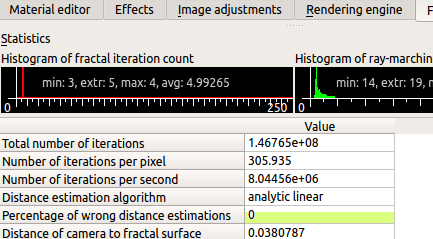
\includegraphics[width=0.5\linewidth]{img/manual/media/mandelboxmenger_statistics.png}

The \emph{Raymarching step multiplier}\index{ray marching!step multiplier} (\emph{Rendering Engine} tab) or
\emph{fudge factor} is set at 0.6, which is good for a hybrid. If I change it to
0.7 the Percentage of Bad DE leaps up to 0.25 and you can see the areas of
quality loss on your image.

Now if we disable the \emph{addCpixel Axis swap Constant Multiplier}, we find we
can now increase the \emph{Raymarching Step Multiplier} to 0.9, and get a faster
render and visually the same quality. So monitoring Percentage of Wrong Distance
Estimations is a guide to managing quality. (Note when doing animations you may
want to drop the Raymarching step down a bit to allow for what might happen
between keyframes.)

MandelboxMenger Hybrids\index{fractal!hybrid} can behave a bit differently to a lot of hybrids, in the
fact that the \emph{Percentage Bad DE} often improves when you zoom in.

\paragraph{Optimizing of \emph{maximum view distance}}\index{ray marching!maximum view distance} Located : Rendering
Engine - Common Rendering settings

It is important to optimize this setting to minimize render time. You can reduce
until the furthest part of the 3D object(s) starts to disappear. However with
animation an allowance should be made for changes between keyframes.

\textbf{Note!} When navigating in Relative step mode, mouse click on
spherical\_inversion, camera zooms out, tand maximum view distance becomes set
on 280. If you don't reset it your render times will be increased.
	

\paragraph{Magic Angle} Benesi Mag Transforms

In mathematics the Magic Angle = 54.7356° .

When rendering basic mag transforms the image does not render parallel to the
standard x,y,z global axis. On the fractal dock, in ``Global parameters'' set
y-axis rotation to 35.2644° (= 90° - 54.7356°). The fractal will then render
parallel to the x-y plane.

\subsubsection{Example of using Transform Menger Fold to make
	Hybrid}\label{example-of-using-transfrom-mengerfold}\index{fractal!hybrid}

\begin{verbatim}[fontsize=\scriptsize]
# Mandelbulber settings file
# version 2.08
# only modified parameters
[main_parameters]
ambient_occlusion_enabled true;
camera -1.528388569045064 -1.23063017895654 -0.0251755516595821;
camera_distance_to_target 0.0004503351519815117;
camera_rotation -14.07789975269277 -44.28785609194563 3.773777260910995;
camera_top 0.2333184436621841 0.6598138513697914 0.7142885869084139;
DE_factor 0.7;
flight_last_to_render 0;
formula_1 1052;
formula_2 1010;
formula_3 1052;
formula_4 1009;
formula_iterations_1 5;
formula_start_iteration_4 45;
formula_stop_iteration_2 12;
formula_stop_iteration_4 5;
fractal_constant_factor 0.9 0.9 0.9;
fractal_enable_4 false;
hdr true;
hybrid_fractal_enable true;
keyframe_last_to_render 0;
main_light_alpha 2.6;
main_light_beta 1.59;
mat1_coloring_palette_offset 46.51;
mat1_coloring_palette_size 255;
mat1_coloring_random_seed 647723;
SSAO_random_mode true;
target -1.528310155903731 -1.230317492741513 -0.02549000429402527;
volumetric_fog_colour_1_distance 3.55841069795292e-06;
volumetric_fog_colour_2_distance 7.116821395905841e-06;
volumetric_fog_distance_factor 7.116821395905841e-06;
[fractal_1]
transf_addition_constantA_000 -0.071633 0 0;
transf_function_enabledy false;
transf_int_1 12;
transf_scale 0.5;
transf_scaleC_1 0;
transf_stop_iterations_1 2;
[fractal_2]
transf_scale3D_333 1.055556 1.027778 0.861111;
[fractal_3]
transf_function_enabledx false;
\end{verbatim}

On this transform UI, the standard menger sponge formula is split into a start
and end function. The simplest way to use this transform is in Hybrid Mode,
having the menger fold transform in slots 1 and 3. In slot 2 place any linear
type formula or transform. (ie more mengers, kifs, mboxes, amazing surf, folds,
rotation , Benesi T1 etc).

In slot 1 disable the stop function
and in slot 3 disable the start function, resulting in a standard menger sponge
with something in the middle.

BTW in fact you can mix around
with the start and stop functions have all enabled if you wish. Generally linear
functions all work well together in making hybrids.

In
Statistics, maximum is approx. 80 iterations. Generally hybrids take longer to
render than standard formulas.
As well as adjusting formula parameters, you
can use the iteration controls to tweak hybrids. In this example the first slot
is set to repeat for 5 iterations before moving to slot 2. Slot 2 is set to stop
at iteration 12, whereas slots 1 and 3 can continue to termination conditions are
met (bailout or maximum number of iterations).

In the example above, slot2 of the hybrid sequenced ended at iteration 12. 12
was chosen because how it fitted into the iteration sequence, as follows:

\begin{itemize}
\item \textbf{Slot 1} x 5 -- iterations: 0, 1, 2, 3, 4 (note first iteration is iteration number 0)
\item \textbf{Slot 2} -- iteration 5
\item \textbf{Slot 3} -- iteration 6
\item \textbf{Slot 1} -- iterations 7, 8, 9, 10, 11
\item \textbf{Slot 2} -- iteration 12 (last use of \textbf{Slot 2})
\end{itemize}

Sequence continues \textbf{Slot 1} x 5, \textbf{Slot 3}, \ldots to bailout.

As you see \textbf{Slot 2} is used only twice in the iteration process. If I had entered 11 instead of 12 for \textbf{Slot 2}'s \emph{stop iterations}, then the slot would have been used only once, if I entered 19 then it would run three times.

\subsection{Q\&A . How do you get different materials on different
	shapes?}\label{qa-.-how-do-you-get-different-materials-on-different-shapes}

This is how I have been doing it.\\[2\baselineskip]\emph{Rectangle at the bottom
	marked A.}\\[2\baselineskip]This is where you~ start a new material or load an
existing.~ The active material is highlighted in blue. Meaning it is active in
the \textbf{material editor} where you create or modify the
material.\\[2\baselineskip]\emph{Rectangle at top left marked
	B.}\\[2\baselineskip]One way to use a material is to go to Global Parameters,
click on the material preview image, and the \textbf{Material Manager} UI will
appear with the materials you have loaded or created. Click on the one you want
to use, then close that UI.\\ Similarly with primitives, click on the material
preview image. And with Boolean Mode each fractal/transform has it's own
material preview image when you scroll down.

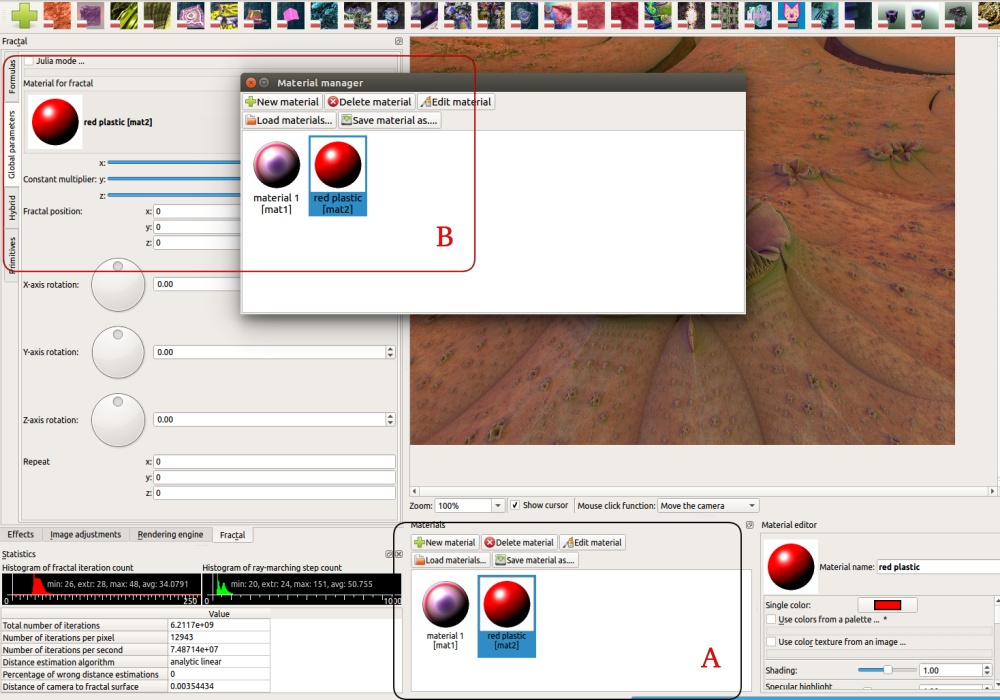
\includegraphics[width=6.69291in,height=4.68465in]{img/manual/media/image32.jpg}

